\chapter{IDEIA GERAL}
\label{conceituacaoEIdeiaGeral} %mudar label
Este capítulo tem como foco expôr o processo de desenvolvimento da nossa pesquisa, e o amadurecimento do tema abordado.

\section{Escolha do tema}
\label{sec: escolhaDoTema}
Durante as eleições de 2014, várias pesquisas foram levantadas em diversas redes sociais sobre a opinião das pessoas a respeito dos atuais candidatos. Analisando essas pesquisas, percebemos que muitas delas, apenas ao comparar o número de menções dos candidatos, não expunham a opinião expressa por trás dessas menções.

Percebemos então que pesquisas em áreas diversas apenas levavam em conta a quantidade de menções, e raramente consideravam se a opinião expressa da pessoa que a fez era positiva, negativa, ou neutra sobre o item mencionado.

Essa realidade nos motivou a desenvolver uma aplicação capaz de gerar uma pesquisa, levando em conta o contexto em que a palavra é encontrada. Tal pesquisa com essa característica poderia mostrar que um número alto de menções nas redes sociais não é garantia de aceitação popular.

No decorrer da pesquisa descobrimos o termo Análise de Sentimento(Seção \ref{sec: analiseSentimento}), que se ajustava com a ideia de analisar as opiniões embutidas nos textos coletados das redes sociais.

Pesquisando mais sobre o assunto, percebemos que o nível de complexidade poderia ser suficiente para dois trabalhos de graduação:
\begin{itemize}
    \item O primeiro sendo responsável por armazenar informações coletadas de redes sociais, de forma organizada e eficiente, em um banco de dados;
    \item O segundo, implementar uma ferramenta que realize a análise de sentimento na língua portuguesa, e aplicá-la nos textos armazenados usando o modelo do primeiro trabalho.
\end{itemize}

Assim, futuros trabalhos nessa área poderão preocupar-se precisamente com a análise em si, sabendo que existem eficientes métodos de pesquisa implementados, e um modelo de banco de dados planejado para este fim, prontos para serem utilizados.

\section{TAZ}
\label{sec: TAZ}
Nossa aplicação Web, denominada TAZ, foi desenvolvida para servir como um framework de extração de dados de redes sociais.

\subsection{Visão geral da aplicação}
\label{subsec: visaoGeralDaAplicacao}
Escolhemos implementar o modelo de banco de dados nesse trabalho, já que a análise de sentimentos depende de informações previamente armazenadas.
Portanto, nossa aplicação deve:
\begin{enumerate}
    \item Receber um tema de pesquisa como entrada;
    \item Aplicar métodos de busca em diversas redes sociais;
    \item Armazenar os textos coletados em um banco de dados modelado especialmente para a aplicação da análise de sentimento.
\end{enumerate}

\begin{figure}[ht]
  \centering
  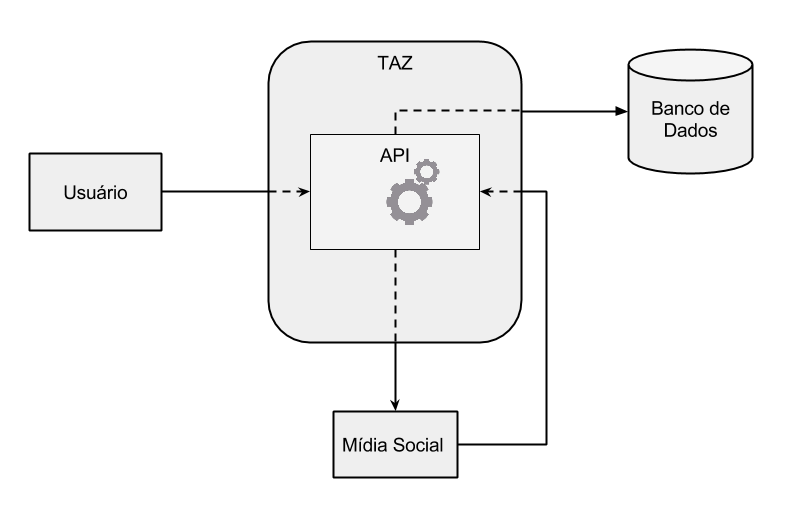
\includegraphics[width=.8\textwidth]{images/esquema}
 
  \caption{Esquema geral da aplicação.}
  \label{fig:esquema}
\end{figure}

\subsection{Termos para pesquisa}
\label{subsec: TermosPesquisa}
Para que o usuário possa definir os termos para pesquisa, foi implementada uma interface web com campos de formulário simples. Através desses campos, o usuário do framework envia para o servidor uma Keyword\footnote{Palavra-chave pela qual será realizada uma pesquisa. Cada resultado possui ao menos uma vez essa palavra no texto} obrigatória e 3 Tags\footnote{Palavra que simboliza um termo relacionado à Keyword. Pode aparecer, mas não obrigatoriamente, nos resultados da pesquisa realizada.} opcionais.

\subsection{Método de busca à rede social}
\label{subsec: MetodoRedeSocial}
Como já mencionado na seção \ref{sec: Redes sociais}, cada rede social tem um objetivo diferente, assim cada API tem métodos de busca distinto que retornam seus objetos correspondentes. Por exemplo, os métodos de busca da API do YouTube são voltados para encontrar vídeos. Já na API do Twitter, os métodos de busca retornam textos. Os métodos de busca da API do Reddit retornam links, que podem apontar para imagens, textos, vídeos, entre outros.
Assim, é necessário uma interface que trate todas essas diferenças e apresente, em um único formato, um método de busca mais abstrato.

\subsection{Modelagem dos resultados}
\label{subsec: ModelagemDosResultados}
Tendo em vista as especificidades de cada rede social e seus métodos, deve-se também adaptar as informações recebidas ao modelo de banco de dados criado para o TAZ.

Este modelo do banco de dados foi idealizado para armazenar características de textos com caráter opinativos, oriundo de quaisquer redes sociais.
Sendo assim, deve ser genérico o suficiente para guardar dados comuns destes textos.

Estudando trabalhos e outras ferramentas de análise de sentimento, consideramos como mais relevantes as seguintes informações:

\begin{itemize}
    \item Texto
    \item Frequência
    \item Fonte
    \item Data postagem
    \item Autor
    \item Palavras pesquisadas
\end{itemize}

Nosso modelo de banco de dados foi projetado para armazenar as informações acima, ficando a cargo do desenvolvedor identificar quais informações da rede social correspondem a cada um dos campos acima.